\documentclass[11pt]{article}
\usepackage[margin=0.7in]{geometry}
\usepackage{amsmath,amssymb}
\usepackage{enumitem}
\usepackage{tikz}
\usepackage{pgfplots}
\pgfplotsset{compat=1.18}
\usepackage{fancyhdr}
\usepackage{parskip}
\setlist[enumerate]{leftmargin=*, itemsep=6pt}
\pagestyle{fancy}
\fancyhf{}
\fancyfoot[L]{\small\textit{en}Vision\textsuperscript{\textregistered} Algebra 2}
\fancyfoot[C]{\small 6-1 Lesson Quiz, short form}
\fancyfoot[R]{\small\thepage}
\renewcommand{\headrulewidth}{0pt}
\newcommand{\choice}[1]{\tikz[baseline=-0.6ex]\node[draw, circle, inner sep=0.6pt, minimum size=3.3mm, font=\scriptsize\bfseries] {#1};\;}
\newcommand{\checkbox}{$\square$\;}
\newcommand{\ansline}[1][3cm]{\rule[-2pt]{#1}{0.4pt}}
\pgfplotsset{quizgrid/.style={
  axis lines=middle, grid=both, grid style={gray!45},
  ticklabel style={font=\scriptsize, fill=white, inner sep=1pt},
  xlabel={$x$}, ylabel={$y$}, axis line style={thick}, clip=true}}

\begin{document}

\noindent\textbf{Name}\; \rule{6cm}{0.4pt} \hfill Period \rule{1.2cm}{0.4pt} \quad Date \rule{2.2cm}{0.4pt}

\vspace{4pt}\noindent\rule{\textwidth}{0.6pt}

\vspace{2pt}\noindent{\LARGE\textbf{6-1 \; Lesson Quiz: Key Features of Exponential Functions}}

\noindent{\small short form \hfill questions keep their Savvas numbers (2, 3, 4); show your work}

\vspace{2pt}\noindent\rule{\textwidth}{0.6pt}

\vspace{4pt}
\textbf{2.} 15,000 blue trout were released into the Meherrin River for a scientific study. The function $f(x)=15{,}000\left(\frac98\right)^x$ represents the number of blue trout after $x$ years. After 5 years, what happens to the population?

\begin{minipage}[t]{0.44\textwidth}
\begin{itemize}[leftmargin=1.2em, itemsep=5pt]
\item[] \choice{A} It decreases by about 2,000.
\item[] \choice{B} It decreases by about 12,000.
\item[] \choice{C} It increases by about 2,000.
\item[] \choice{D} It increases by about 12,000.
\end{itemize}
\end{minipage}\hfill
\begin{minipage}[t]{0.52\textwidth}
Show your work: $f(5)=\ansline[3.5cm]$

\vspace{14pt}
Change after 5 years: \ansline[3.6cm]
\end{minipage}

\vspace{8pt}\noindent\rule{\textwidth}{0.4pt}

\vspace{4pt}
\textbf{3.} For the function $f(x)=\left(\frac12\right)\cdot6^x$, identify the domain, range, $y$-intercept, and asymptote. Write one of the given phrases or values in each blank.

\vspace{2pt}
\noindent\fbox{\parbox{\dimexpr\textwidth-2\fboxsep-2\fboxrule}{\centering
linear \qquad quadratic \qquad exponential \qquad all real numbers \qquad 0.5 \qquad 0 \qquad 0}}

\vspace{8pt}
\begin{tabular}{@{}l@{\quad}l@{\qquad\qquad}l@{\quad}l@{}}
Domain: & \ansline[4cm] & $y$-intercept: & \ansline[3cm] \\[12pt]
Range: & $\{y\mid y>\ansline[1.6cm]\}$ & Asymptote: & $y=\ansline[2cm]$ \\[12pt]
Function type: & \ansline[4cm] & & \\
\end{tabular}

\vspace{6pt}\noindent\rule{\textwidth}{0.4pt}

\vspace{4pt}
\begin{minipage}[t]{0.44\textwidth}
\textbf{4.} The rabbit population of Springfield, Ohio, was 144,000 in 2016. It is expected to decrease by about 7.2\% per year. Write and graph the exponential decay function of the rabbit population, $P(t)$.

\vspace{14pt}
$P(t)=\ansline[2.6cm]\,\big(\ansline[1.8cm]\big)^t$

\vspace{14pt}
Decay factor: \ansline[2cm]

\vspace{14pt}
What does $t$ count? \ansline[3.4cm]
\end{minipage}\hfill
\begin{minipage}[t]{0.54\textwidth}
\vspace{-4pt}
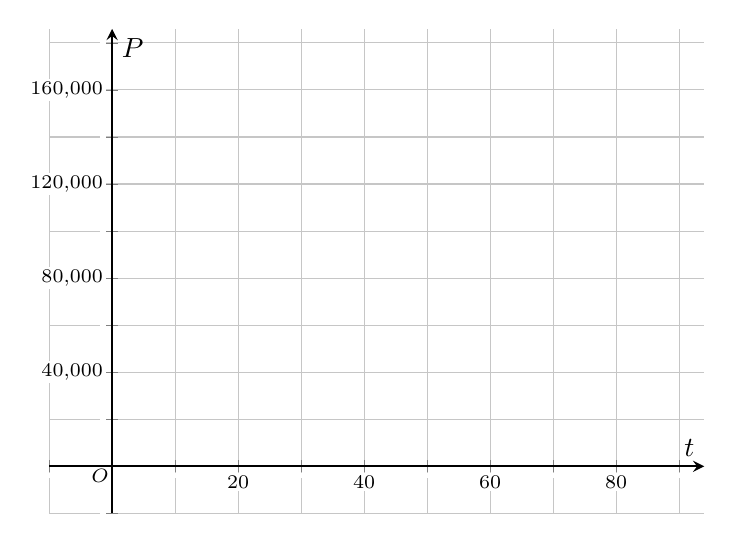
\begin{tikzpicture}
% TE window t -10 to 90 (grid 10, labels 20-80), P -20,000 to 180,000 (grid 20,000, labels 40,000-160,000); O at origin
\begin{axis}[quizgrid, xmin=-10, xmax=94, ymin=-20000, ymax=186000,
  xtick={-10,0,...,90}, ytick={-20000,0,...,180000},
  xticklabels={,,,20,,40,,60,,80,},
  yticklabels={,,,40{,}000,,80{,}000,,120{,}000,,160{,}000,},
  scaled y ticks=false,
  x=0.08cm, y=0.000033cm, xlabel={$t$}, ylabel={$P$}]
\node[font=\scriptsize, inner sep=1pt, anchor=north east] at (axis cs:0,0) {$O$};
\end{axis}
\end{tikzpicture}
\end{minipage}

\vfill
\noindent\textbf{Scoring:} Question 3 and Question 4 are 10 points each. Question 2 is a bonus of up to 5 points. Total out of 20.

\newpage
\noindent{\LARGE\textbf{6-1 Lesson Quiz, short form: answer key}}

\vspace{4pt}\noindent\rule{\textwidth}{0.6pt}

\begin{enumerate}
\item[\textbf{2.}] \textbf{D, it increases by about 12,000.} The base $\frac98=1.125>1$, so the population grows. $f(5)=15{,}000\left(\frac98\right)^5=15{,}000\cdot\frac{59{,}049}{32{,}768}\approx27{,}030$, and $27{,}030-15{,}000\approx12{,}030$. Choice C is a common slip: $15{,}000(0.125)\approx1{,}900$ is one year's increase, not five. Savvas quiz item 2, DOK 2, Skills Review and Practice F14. Taught by Example 3B (evaluate the model at a later time) and Try It 3b-c. \textbf{Bonus 5:} 3 for D, 2 for shown work ($f(5)\approx27{,}000$ or the difference).
\item[\textbf{3.}] \textbf{Domain: all real numbers; Range: $\{y\mid y>0\}$; $y$-intercept: $0.5$; Asymptote: $y=0$; Function type: exponential.} $a=\frac12$ is the $y$-intercept because $6^0=1$; $b=6>1$, so the graph rises from the $x$-axis on the left. Savvas quiz item 3, DOK 2, F13. Taught by Example 1 (Try It 1 is the same five features). \textbf{10 points:} 2 per correct blank.
\item[\textbf{4.}] \textbf{$P(t)=144{,}000(0.928)^t$.} Decay factor $1-0.072=0.928$; $t$ is years since 2016. Graph: starts at the filled point $(0,144{,}000)$ and decreases toward the $t$-axis (asymptote $P=0$), passing near $(10,68{,}000)$, $(20,32{,}000)$, $(40,7{,}000)$; the TE answer graph ends near $(90,0)$. Savvas quiz item 4, DOK 2, F13 and F14. Taught by Example 3 and the decay model box (Try It 3 is the same decay shape). \textbf{10 points:} 3 for 144,000, 4 for 0.928, 3 for a decreasing curve through $(0,144{,}000)$ that approaches but does not cross the $t$-axis. A student who writes $0.072$ as the base loses the 4 points (it is the rate, not the decay factor; concept summary Common Error).
\end{enumerate}

\textbf{Items left off this form} (available for a retake or Form B): Savvas item 1, the function for $f(x)=3^x$ after a vertical stretch by a factor of 8 and a reflection across the $x$-axis (answer D, $g(x)=-8\cdot3^x$; DOK 2, F28; it is the cut Example 2 and Lesson 1-2 transformations); Savvas item 5, which function has a greater growth factor than the graphed one through $(0,16)$, $(2,36)$, $(3,54)$ (answer A, $f(x)=\left(\frac32\right)\cdot3^x$, because the graph's growth factor is $\frac{54}{36}=1.5$ and $3>1.5$; choice B has the same factor 1.5; DOK 2, F14; it is the cut Example 5). Item 5's graph could be redrawn from the TE description; it is left off because no kept Example teaches it, not because of the figure (Example 1's study tip, ratio of consecutive $y$-values $=b$, is the one-minute bridge if the teacher puts it back).

\textbf{IXL replacement:} SmartScore 70 or above on EFD, U7P, DBW and TYQ replaces this quiz with 20/20.

\end{document}
